%% LyX 2.0.6 created this file.  For more info, see http://www.lyx.org/.
%% Do not edit unless you really know what you are doing.
\documentclass[english]{article}
\usepackage[T1]{fontenc}
\usepackage[utf8]{luainputenc}
\usepackage{geometry}
\geometry{verbose,tmargin=1.5cm,bmargin=1.5cm,lmargin=1.5cm,rmargin=1.5cm}
\usepackage{booktabs}
\usepackage{amstext}
\usepackage{amssymb}
\usepackage{graphicx}

\makeatletter

%%%%%%%%%%%%%%%%%%%%%%%%%%%%%% LyX specific LaTeX commands.
%% Because html converters don't know tabularnewline
\providecommand{\tabularnewline}{\\}

\makeatother

\usepackage{babel}
\begin{document}

\part*{Lineare Algebra}


\section*{Vektorgeometrie}


\subsection*{Berechnung des Skalarprodukts}
\begin{verse}
$\vec{a}\bullet\vec{b}=\left(\begin{array}{c}
a_{x}\\
a_{y}\\
a_{z}
\end{array}\right)\bullet\left(\begin{array}{c}
b_{x}\\
b_{y}\\
b_{z}
\end{array}\right)=a_{x}b_{x}+a_{y}b_{y}+a_{z}b_{z}$
\end{verse}

\subsection*{Berechnung des Zwischenwinkels zweier Vektoren}
\begin{verse}
$\cos\measuredangle(\vec{v},\vec{w})=\frac{\vec{v}\bullet\vec{w}}{\left|\vec{v}\right|\cdot\left|\vec{w}\right|}\Rightarrow\measuredangle(\vec{v},\vec{w})=\arccos\frac{\vec{v}\bullet\vec{w}}{\left|\vec{v}\right|\cdot\left|\vec{w}\right|}$

$\vec{v}\bullet\vec{w}=\left|\vec{v}\right|\cdot\left|\vec{w}\right|\cdot cos\measuredangle(\vec{v},\vec{w})$
\end{verse}

\subsection*{Aussage des Skalarprodukts 0}
\begin{verse}
$\vec{v}\perp\vec{w}\Leftrightarrow\vec{v}\bullet\vec{w}=0$
\end{verse}
Nullvektoren stehen senkrecht zu allen Vektoren


\subsection*{Berechnung der Länge eines Vektors}
\begin{verse}
$\vec{a}=\left(\begin{array}{c}
a_{1}\\
a_{2}\\
a_{3}
\end{array}\right)$

$\left|\vec{a}\right|=\sqrt{a_{1}^{2}+a_{2}^{2}+a_{3}^{2}}=\sqrt{\vec{a}\bullet\vec{a}}$

$\vec{a}\bullet\vec{a}=a_{1}^{2}+a_{2}^{2}+a_{3}^{2}=\left|\vec{a}\right|^{2}$
\end{verse}

\subsection*{Satz des Pythagoras}


\subsubsection*{Im Dreieck}
\begin{verse}
\begin{tabular}{c}
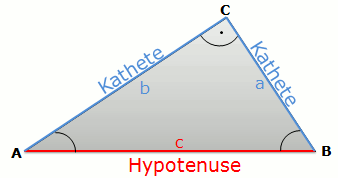
\includegraphics[width=6.279cm]{pythagoras}\tabularnewline
$a^{2}+b^{2}=c^{2}$\tabularnewline
\end{tabular}
\end{verse}

\subsubsection*{Mit Vektoren}
\begin{verse}
\begin{tabular}{c}
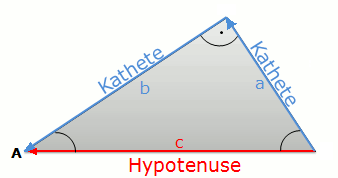
\includegraphics[width=6.279cm]{pythagoras_vektoren}\tabularnewline
\end{tabular}

$\vec{b}=\vec{c}-\vec{a}$

$\vec{c}=\vec{a}+(\vec{c}-\vec{a})$

$\left|\vec{c}\right|=\sqrt{\vec{c}\bullet\vec{c}}=\sqrt{(\vec{a}+(\vec{c}-\vec{a})\bullet(\vec{a}+(\vec{c}-\vec{a}))}=\sqrt{(\vec{a}+\vec{b})\bullet(\vec{a}+\vec{b})}$

$=\sqrt{\vec{a}\bullet\vec{a}+\vec{a}\bullet\vec{b}+\vec{c}\bullet\vec{b}+\vec{b}\bullet\vec{b}}=\sqrt{\left|\vec{a}\right|^{2}+0+0+\left|\vec{b}\right|^{2}}=\sqrt{\left|\vec{a}\right|^{2}+\left|\vec{b}\right|^{2}}$
\end{verse}

\subsection*{Cosinussatz}
\begin{verse}
\begin{tabular}{c}
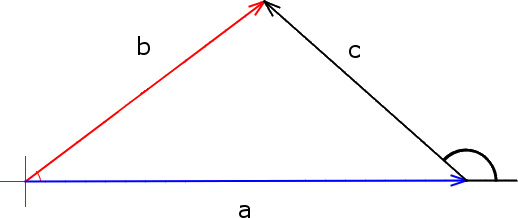
\includegraphics[width=9cm]{Kosinussatz}\tabularnewline
\end{tabular}

$\vec{c}=\vec{b}-\vec{a}$

$\left|\vec{b}\right|^{2}=\vec{b}\bullet\vec{b}=(\vec{a}+\vec{c})\bullet(\vec{a}+\vec{c})=\vec{a}\bullet\vec{a}+\vec{a}\bullet\vec{c}+\vec{c}\bullet\vec{a}+\vec{c}\bullet\vec{c}$

$=\left|\vec{a}\right|^{2}+2\cos\measuredangle(\vec{a},\vec{c})\cdot\left|\vec{a}\right|\cdot\left|\vec{c}\right|+\left|\vec{c}\right|^{2}$

$(=\left|\vec{a}\right|^{2}-2\cos(180^{o}-\measuredangle)\cdot\left|\vec{a}\right|\cdot\left|\vec{c}\right|+\left|\vec{c}\right|^{2})$
\end{verse}
Daraus folgt:
\begin{verse}
$a^{2}+c^{2}-2ac\cdot\cos(\beta)=b^{2}$
\end{verse}

\subsection*{Orthogonalprojektion}
\begin{verse}
\begin{tabular}{c}
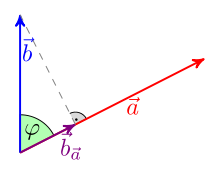
\includegraphics[width=5cm]{Orthogonalprojektion}\tabularnewline
\end{tabular}\end{verse}
\begin{enumerate}
\item Einheitsvektor in $\vec{a}$-Richtung $=\frac{1}{\left|\vec{a}\right|}\cdot\vec{a}=\vec{a_{1}}(=\vec{b_{a}})$
\item $\vec{b}\bullet\vec{a_{1}}=\left|\vec{b}\right|\cdot\left|\vec{a_{1}}\right|\cdot\cos\measuredangle(\vec{b},\vec{a_{1}})=\left|\vec{b}\right|\cdot\cos\measuredangle(\vec{b},\vec{a_{1}})$ 
\item $\left|\vec{b}\right|\cdot\cos\measuredangle(\vec{b},\vec{a_{1}})\cdot\frac{\vec{a}}{\left|\vec{a}\right|}=(\vec{b}\bullet\frac{\vec{a}}{\left|\vec{a}\right|})\bullet\frac{\vec{a}}{\left|\vec{a}\right|}=(\vec{b}\bullet\frac{\vec{a}}{\left|\vec{a}\right|^{2}})\bullet\vec{a}$
\end{enumerate}

\subsection*{Kreuzprodukt}

$\left(\begin{array}{c}
a_{1}\\
a_{2}\\
a_{3}
\end{array}\right)x\left(\begin{array}{c}
b_{1}\\
b_{2}\\
b_{3}
\end{array}\right)=\left(\begin{array}{c}
a_{2}\cdot b_{3}-a_{3}\cdot b_{2}\\
a_{3}\cdot b_{1}-a_{1}\cdot b_{3}\\
a_{1}\cdot b_{2}-a_{2}\cdot b_{1}
\end{array}\right)$


\subsection*{Parameterdarstellung}

Gerade = Aufpunkt + Faktor {*} Vektor
\begin{verse}
$g:\left(\begin{array}{c}
x\\
y\\
z
\end{array}\right)=\left(\begin{array}{c}
10\\
3\\
-12
\end{array}\right)+s\left(\begin{array}{c}
-5\\
1\\
-3
\end{array}\right)$
\end{verse}
Ebene = Aufpunkt + 1.Faktor {*} 1.Vektor + 2.Faktor {*} 2. Vektor
\begin{verse}
\emph{$E:\left(\begin{array}{c}
x\\
y\\
z
\end{array}\right)=\left(\begin{array}{c}
10\\
3\\
-12
\end{array}\right)+s\left(\begin{array}{c}
-5\\
1\\
-3
\end{array}\right)+t\left(\begin{array}{c}
4\\
9\\
1
\end{array}\right)$}
\end{verse}

\subsection*{Koordinatengleichung der Ebene}

Parameterdarstellung:
\begin{verse}
\emph{$E:\left(\begin{array}{c}
x\\
y\\
z
\end{array}\right)=\left(\begin{array}{c}
1\\
-1\\
2
\end{array}\right)+s\left(\begin{array}{c}
-3\\
1\\
1
\end{array}\right)+t\left(\begin{array}{c}
2\\
2\\
-4
\end{array}\right)$}\end{verse}
\begin{itemize}
\item Kreuzprodukt der Vektoren berechnen\end{itemize}
\begin{verse}
$\left(\begin{array}{c}
-3\\
1\\
1
\end{array}\right)x\left(\begin{array}{c}
2\\
2\\
-4
\end{array}\right)=\left(\begin{array}{c}
-6\\
-10\\
-8
\end{array}\right)=\left(\begin{array}{c}
3\\
5\\
4
\end{array}\right)$\end{verse}
\begin{itemize}
\item Gleichung aufstellen\end{itemize}
\begin{verse}
$3x+5y+4z=0$\end{verse}
\begin{itemize}
\item Aufpunkt einsetzen\end{itemize}
\begin{verse}
$3-5+8=6$

$\Rightarrow3x+5y+4z=6$

$\Rightarrow3x+5y+4z-6=0$
\end{verse}

\section*{Beispiele}


\subsection*{Schnittgerade zweier Ebenen}

Gegeben:
\begin{verse}
$E_{1}=\left(\begin{array}{c}
3\\
1\\
2
\end{array}\right)+u\left(\begin{array}{c}
1\\
0\\
0
\end{array}\right)+v\left(\begin{array}{c}
0\\
1\\
1
\end{array}\right)$

$E_{2}=\left(\begin{array}{c}
4\\
2\\
0
\end{array}\right)+u\left(\begin{array}{c}
0\\
2\\
-1
\end{array}\right)+v\left(\begin{array}{c}
0\\
0\\
1
\end{array}\right)$\end{verse}
\begin{itemize}
\item Normalen der Ebenen bestimmen (Kreuzprodukt)\end{itemize}
\begin{verse}
$n_{1}=\left(\begin{array}{c}
1\\
0\\
0
\end{array}\right)x\left(\begin{array}{c}
0\\
1\\
1
\end{array}\right)=\left(\begin{array}{c}
0\\
-1\\
1
\end{array}\right)$

$n_{1}=\left(\begin{array}{c}
4\\
2\\
0
\end{array}\right)x\left(\begin{array}{c}
0\\
2\\
-1
\end{array}\right)=\left(\begin{array}{c}
2\\
0\\
0
\end{array}\right)$\end{verse}
\begin{itemize}
\item Gleichungen für Normalen aufstellen und Aufpunkte einsetzen\end{itemize}
\begin{verse}
$\left(\begin{array}{c}
0\\
-1\\
1
\end{array}\right)\Rightarrow-y+z=0\Rightarrow-1+2=1\Rightarrow-x+z=1$

$\left(\begin{array}{c}
2\\
0\\
0
\end{array}\right)\Rightarrow2x=0\Rightarrow8=8\Rightarrow2x=8$\end{verse}
\begin{itemize}
\item Normalen zu den Normalen bestimmen\end{itemize}
\begin{verse}
$r=\left(\begin{array}{c}
0\\
-1\\
1
\end{array}\right)x\left(\begin{array}{c}
2\\
0\\
0
\end{array}\right)=\left(\begin{array}{c}
0\\
2\\
2
\end{array}\right)$

$\Rightarrow0x+2x+2z=0$\end{verse}
\begin{itemize}
\item Aufpunkt bestimmen\end{itemize}
\begin{verse}
Aufpunkt so wählen, dass er beide Gleichungen erfüllt

$0x-y-z=1$

$2x+0y+0z=8$

$\Rightarrow\left(\begin{array}{c}
4\\
1\\
2
\end{array}\right)$\end{verse}
\begin{itemize}
\item Parameter Darstellung\end{itemize}
\begin{verse}
$r=\left(\begin{array}{c}
4\\
1\\
2
\end{array}\right)+t\left(\begin{array}{c}
0\\
2\\
2
\end{array}\right)$
\end{verse}

\subsection*{Normalstehende Ebene}

Gegeben
\begin{verse}
$E:\; x+2y+2z-4=0$

$A(-1/-2/0),\; B(1/1/2)$
\end{verse}
Gesucht: Ebene die Normla zur gegeben Ebene liegt, und durch die Punkt
A und B geht.
\begin{itemize}
\item u, v berechnen\end{itemize}
\begin{verse}
$u=n=\left(\begin{array}{c}
1\\
2\\
2
\end{array}\right)$ $v=B-A=\left(\begin{array}{c}
1\\
1\\
2
\end{array}\right)-\left(\begin{array}{c}
-1\\
-2\\
0
\end{array}\right)=\left(\begin{array}{c}
2\\
3\\
2
\end{array}\right)$

$E:\left(\begin{array}{c}
x\\
y\\
z
\end{array}\right)=A+s*u+t*v=$

$E:\left(\begin{array}{c}
x\\
y\\
z
\end{array}\right)=\left(\begin{array}{c}
-1\\
-2\\
0
\end{array}\right)+s\left(\begin{array}{c}
1\\
2\\
2
\end{array}\right)+t\left(\begin{array}{c}
2\\
3\\
2
\end{array}\right)$\end{verse}
\begin{itemize}
\item Berechnen der Koordinatengleichung\end{itemize}
\begin{verse}
$n_{2}=u\times v=\left(\begin{array}{c}
1\\
2\\
2
\end{array}\right)\times\left(\begin{array}{c}
2\\
3\\
2
\end{array}\right)=\left(\begin{array}{c}
-2\\
2\\
-1
\end{array}\right)$ 

$-2x+2y-z=0$\end{verse}
\begin{itemize}
\item Aufpunkt einsetzen (A ist der Aufpunkt)\end{itemize}
\begin{verse}
$-2*(-1)+2*(-2)-0=-2$

$\Rightarrow-2x+2y-z+2=0$
\end{verse}

\subsection*{Drehung (Drehmatrix)}

$A_{D(45\text{°) }}=\left(\begin{array}{cc}
cos(45\text{°)} & -sin(45\text{°)}\\
sin(45\text{°)} & cos(45\text{°)}
\end{array}\right)$


\subsection*{Spiegelung}
\begin{itemize}
\item An x-Achse $\left(\begin{array}{cc}
1 & 0\\
0 & -1
\end{array}\right)$
\item An y-Achse $\left(\begin{array}{cc}
-1 & 0\\
0 & 1
\end{array}\right)$
\end{itemize}

\subsubsection*{An Geraden 2x -5y = 0 (Wenn die Gerade nicht durch den Nullpunkt
geht, gehts nicht, nicht linear)}

1. Normale der Gerade bestimmen:
\begin{verse}
$n=\left(\begin{array}{c}
2\\
-5
\end{array}\right)$, da $n\bullet r=0$, ist der Vektor $r=\left(\begin{array}{c}
5\\
2
\end{array}\right)$(Vektor umdrehen und eine Zahl negieren)
\end{verse}
2. Nun kann eine Gleichung aufgestellt werden:
\begin{verse}
$A(n*r)=(-n*r)$, dies kann man schreiben als A{*}B =C
\end{verse}
3. Nun kann auf beiden Seiten von rechts mit $B^{-1}$multipliziert
werden und man erhält:
\begin{verse}
$A=C*B^{-1}$resp $A=(-n*r)*(n*r)^{-1}$,
\end{verse}
4. Da wir n und r kennen, können wir nun die klammern durch Matrizen
ersetzen
\begin{verse}
$A=\left(\begin{array}{cc}
-2 & 5\\
5 & 2
\end{array}\right)*\left(\begin{array}{cc}
2 & 5\\
-5 & 5
\end{array}\right)^{-1}$
\end{verse}
5. Nun kann es ausgerechnet werden (--> Gausches Eliminationsverfahren
für Invertierung)
\end{document}
